% -*- coding: utf-8 -*-

\documentclass[12pt, a4paper, twosides]{report}
\usepackage[italian]{babel}
\usepackage{ucs}
\usepackage[utf8x]{inputenc} 
\frenchspacing
\usepackage{graphicx}
\usepackage[hmargin=2cm, vmargin=2cm, a4paper]{geometry}
\usepackage{enumitem}
\usepackage{url}
\usepackage{listings}
\usepackage{hyperref}
\usepackage{fancyhdr}
\usepackage[Bjornstrup]{fncychap}

% linea sopra
\makeatletter
\def\cleardoublepage{\clearpage\if@twoside \ifodd\c@page\else
		\hbox{}
		\vspace*{\fill}
		\vspace{\fill}
		\thispagestyle{empty}
		\newpage
		\if@twocolumn\hbox{}\newpage\fi\fi\fi}
\makeatother
 
\pagestyle{fancy}
\renewcommand{\chaptermark}[1]{\markboth{#1}{}}
\renewcommand{\sectionmark}[1]{\markright{\thesection\ #1}}
\fancyhf{}
\fancyhead[L,R]{\scshape\thepage}
\fancyhead[L]{\scshape\footnotesize\nouppercase{\rightmark}}
\renewcommand{\headrulewidth}{0.5pt}
\renewcommand{\footrulewidth}{0pt}
\addtolength{\headheight}{4pt}

\lstset{
	basicstyle=\footnotesize,       % the size of the fonts that are used for the code
	% numbers=left,                   % where to put the line-numbers
	numberstyle=\footnotesize,      % the size of the fonts that are used for the line-numbers
	stepnumber=2,                   % the step between two line-numbers. If it's 1 each line will be numbered
	numbersep=5pt,                  % how far the line-numbers are from the code
	backgroundcolor=\color{white},  % choose the background color. You must add \usepackage{color}
	showspaces=false,               % show spaces adding particular underscores
	showstringspaces=false,         % underline spaces within strings
	showtabs=false,                 % show tabs within strings adding particular underscores
	frame=single,                   % adds a frame around the code
	tabsize=4,                      % sets default tabsize to 2 spaces
	captionpos=b,                   % sets the caption-position to bottom
	breaklines=true,                % sets automatic line breaking
	breakatwhitespace=false,        % sets if automatic breaks should only happen at whitespace
	escapeinside={\%*}{*)}          % if you want to add a comment within your code
}
\renewcommand{\lstlistlistingname}{Elenco dei codici}
\renewcommand{\lstlistingname}{Codice}

\hypersetup{
	colorlinks=true,
	linkcolor=blue
}

\begin{document}

\title{\null \vspace{\stretch{1}}
  \Huge{Implementazione di un SAT solver parallelo basato sull'algoritmo DPLL}
  \\[\baselineskip]
  \Large{Esame di Applicazioni e Calcolo in Rete, Corso Avanzato\\
         A.A. 2007/08\\
         [\baselineskip]
         Corso di Laurea in Informatica\\Università degli Studi di Perugia}\\
  [\baselineskip]
  
\includegraphics[width=.3\textwidth]{unipg.png}\\[\baselineskip]
\vspace{\stretch{1}} \null}
\author{Paolo Bernardi}

\maketitle
\thispagestyle{empty}
\newpage

\setlength{\parskip}{0.5em}
\setlength{\parindent}{0em}


\tableofcontents

\chapter{La teoria}

\section{Il problema SAT}

SAT è l'abbreviazione della parola inglese “Satisfiability” ed è associata al problema della \textit{soddisfacibilità booleana} che è riassumibile nel seguente quesito: data una formula booleana, esiste un assegnamento per le variabili che compaiono in essa tale da renderla vera? Si tratta di un \textit{problema decisionale} la cui risposta è affermativa o negativa; nel primo caso si dice che la formula è soddisfacibile (SAT), nel secondo si dice che è insoddisfacibile (UNSAT).

Il problema SAT è anche conosciuto come \textit{soddisfacibilità proposizionale}; questo nome sottolinea i tipi di operatori booleani utilizzabili, ovvero quelli del calcolo proposizionale: congiunzione (\verb|and|), disgiunzione (\verb|or|), negazione (\verb|not|) e implicazione. Esistono anche formulazioni di SAT che aggiungono altri operatori ed altri tipi di vincoli da rispettare, come disuguaglianze lineari, ma non sono argomento di questo elaborato.

Nonostante SAT abbia come dominio l'insieme di tutte le formule booleane, nella pratica è usuale occuparsi soltanto di \textit{congiunzioni di clausole}. Una clausola è a sua volta una \textit{disgiunzione di letterali} ed un letterale è una \textit{variabile booleana, eventualmente negata}. Questo particolare tipo di formule booleane viene detto essere in \textit{forma normale congiuntiva} (conjunctive normal form, CNF). Un'esempio di formula in CNF è il seguente:

\begin{center}
\verb|(a or b or c) and (d or (not a)) and (not b)|
\end{center}

In questo caso, ad esempio, \verb|a|, \verb|b|, \verb|c|, \verb|d|, \verb|(not a)| e \verb|(not b)| sono dei letterali; \verb|(a or b or c)| è una clausola al pari di \verb|(d or (not a))| e \verb|(not b)|, anche se quest'ultima è formata da un solo elemento. Vincolare un algoritmo di risoluzione per SAT a lavorare soltanto con formule in CNF \textit{non è limitativo nella pratica} perché qualsiasi formula booleana può essere ricondotta in CNF in un tempo polinomiale. Tutti gli algoritmi per risolvere SAT lavorano con formule in CNF e quanto verrà descritto in questo elaborato non farà eccezione.

SAT fa parte dei problemi \textit{NP-completi}; è stato il primo di questa categoria ad essere scoperto, nel 1971 da Stephen Cook. I problemi NP sono caratterizzati dal fatto che fino ad ora non si conoscono algoritmi che li risolvano in tempo polinomiale ma esistono banali algoritmi polinomiali per verificare la correttezza di un risultato già calcolato\footnote{Questa caratteristica è spesso indicata dicendo che i problemi NP hanno un certificato polinomiale.}. I problemi NP-completi come SAT sono un sottoinsieme dei problemi NP la cui caratteristica è che ognuno di loro è riducibile in tempo polinomiale ad un qualsiasi altro problema dello stesso insieme. Come conseguenza, un algoritmo per risolvere velocemente SAT è utilizzabile per risolvere velocemente un \textit{qualsiasi altro problema NP-completo}.

In effetti SAT è un problema particolarmente importante e studiato nel tempo proprio per la sua vasta serie di applicazioni; in particolare è utilizzato nell'ambito della verifica automatica dei circuiti (anche complessi, come quelli dei microprocessori) e dei programmi. Esistono perfino delle competizioni a livello mondiale tra i diversi SAT solver svolte all'interno di convegni sull'argomento della risoluzione booleana.




\section{Il backtracking}

Un modo banale per risolvere i problemi decisionali, tra cui SAT, è quello di esplorare tutte le possibili soluzioni e fornire risposta affermativa soltanto se ce n'è \textit{almeno una} che soddisfi i vincoli del problema. Nel caso di SAT lo spazio delle soluzioni è dato dai \textit{possibili assegnamenti delle variabili} che compaiono nella formula booleana presa in considerazione; ciascuna serie di assegnamenti può essere rappresentata da un vettore avente tanti elementi quante sono le variabili booleane.

La tecnica del backtracking consiste in una \textit{visita} in profondità di un albero avente come nodi tutti i possibili vettori degli assegnamenti, anche parziali, a partire dalla radice con il vettore vuoto fino alle foglie, che sono assegnamenti totali. Ad esempio, per una formula avente come variabili \verb|a| e \verb|b| l'albero appena descritto è il seguente:

\begin{figure}[ht]
\begin{center}
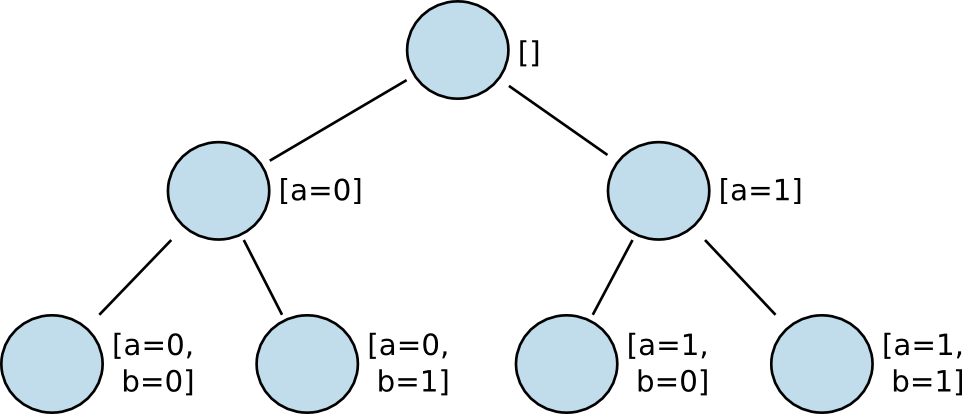
\includegraphics[width=0.8\textwidth]{albero.png}
\end{center}
\caption{L'albero degli assegnamenti parziali generato da una formula booleana con variabili a e b.}
\end{figure}

Si usa la visita in profondità perché è quella che arriva ad esaminare le foglie dell'albero il prima possibile e qualora una foglia sia una soluzione \textit{si può interrompere il processo} tralasciando il resto dell'albero.

\begin{figure}[ht]
\begin{center}
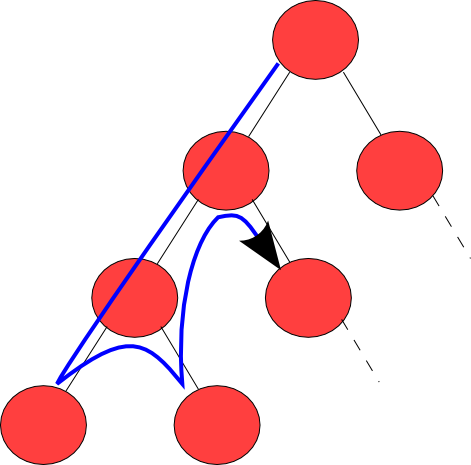
\includegraphics[width=0.5\textwidth]{depthfirst.png}
\end{center}
\caption{La visita in profondità tende a raggiungere subito le foglie dell'albero per poi tornare sui suoi passi.}
\end{figure}

Ovviamente il backtracking ha una \textit{complessità temporale esponenziale} rispetto al numero delle variabili di una formula; in particolare, se queste sono $n$ i nodi dell'albero degli assegnamenti saranno $2^{n}-1$ e nel caso peggiore, ovvero quando la formula non è soddisfacibile, \textit{bisogna visitarli tutti}. La complessità spaziale di questo algoritmo è invece contenuta perché i nodi dell'albero degli assegnamenti possono essere generati man mano che sono necessari ed una volta esaminato tutto il sotto-albero di cui sono radice \textit{possono essere eliminati} dalla memoria.





\section{La procedura DPLL}

DPLL, acronimo di Davis-Putnam-Logemann-Loveland, è il nome di un'algoritmo inventato nel 1962 da questi quattro ricercatori che è ancora oggi alla base dei più efficenti programmi per la risoluzione del problema SAT.

La procedura DPLL è un miglioramento del generico backtracking che sfrutta alcune \textit{peculiarità del problema SAT}. In particolare, grazie ad alcune proprietà dell'algebra booleana, consente, sotto particolari condizioni, di \textit{assegnare un valore fisso} ad una variabile, invece di provarli entrambi; le due regole che fanno questo sono:

\begin{description}
\item[Asserzione:] se ci sono \textit{clausole formate da una sola variabile} si deve per forza assegnarle il valore VERO o, se questa è negata, FALSO. Questo perché, poiché le clausole sono legate tra loro dall'operatore \verb|and|, assegnare alla variabile il valore opposto renderebbe automaticamente falsa tutta la formula a prescindere dai valori delle altre variabili.

\item[Letterale puro:] se una variabile compare, in tutta la formula, \textit{sempre positiva o sempre negata} le si può assegnare rispettivamente il valore di VERO o FALSO. Questo perché nelle singole clausole questa variabile è legata alle altre mediante l'operatore \verb|or| ed assegnarle il valore opposto la renderebbe inutile ai fini della verità di tutte le clausole in cui essa compare.
\end{description}

Inoltre, la procedura DPLL consente di \textit{determinare se una formula sia soddisfacibile o meno anche con assegnamenti parziali}, invece di aspettare di avere assegnamenti totali (le foglie dell'albero). Per ottenere questo effetto la DPLL \textit{semplifica} la formula originaria da valutare man mano che vengono assegnati dei valori alle variabili;  ovviamente la formula semplificata è \textit{equivalente} a quella originale, ai fini del problema da risolvere. Questo processo di semplificazione implica che i nodi dell'albero degli assegnamenti dovranno contenere sia gli assegnamenti parziali o totali delle variabili, sia la formula, eventualmente semplificata, associata all'assegnamento di quel particolare nodo. Le regole per semplificare una formula sulla base delle valutazioni correnti sono:

\begin{description}
\item[Sussunzione]: se una clausola contiene una \textit{variabile positiva con valore VERO} o una \textit{variabile negata con valore FALSO}, questa clausola può essere eliminata dalla formula; in effetti, essendo una clausola una serie di \verb|or|, basta che un termine sia vero per renderla vera nel complesso.

\item[Risoluzione unitaria]: se una clausola contiene una \textit{variabile positiva con valore FALSO} o una \textit{variabile negata con valore VERO}, questa variabile può essere eliminata dalla clausola perché non contribuirebbe a renderla vera.
\end{description}

La regola di sussunzione, cancellando clausola dopo clausola, potrebbe portare ad una \textit{formula priva di clausole}; se ciò avviene, la formula originale è \textit{soddisfacibile}. La regola di risoluzione unitaria invece potrebbe portare all'assurdo di una formula contenente una \textit{clausola senza variabili}: in questo caso, l'assegnamento parziale corrente \textit{non soddisfa} la formula e invece di provare a continuare esaminando le variabili non ancora assegnate si ritorna indietro e si provano nuovi valori per le variabili già assegnate che hanno portato a questo risultato negativo.

Ovviamente se nessuna delle regole sopra citate può essere applicata si procede come con il normale backtracking, ovvero si sceglie una variabile non assegnata e si prova con \textit{entrambi} i valori; questa operazione è chiamata regola di \textbf{sdoppiamento}.





\section{Parallelizzare la DPLL}

Le regole della DPLL compiono tutto sommato operazioni semplici e veloci; la degenerazione esponenziale nel tempo è data dalla necessità di dover applicare comunque lo sdoppiamento. Questa osservazione suggerisce di applicare un \textit{parallelismo di grana grossa}. Il punto più naturale per farlo è proprio quando avviene lo sdoppiamento.

L'implementazione parallela della procedura DPLL descritta nel presente elaborato fa proprio questo: il processo master inizia ad esplorare l'albero degli assegnamenti mediante le regole della DPLL; qualora si presenti la necessità di uno sdoppiamento, controlla se c'è \textit{almeno un worker libero} ed eventualmente gli affida il compito di esplorare una delle due alternative in vece sua; in questo modo, fin tanto che ci sono worker liberi, il master può evitare il continuo raddoppiarsi del suo spazio di ricerca.

A regime, sia i worker che il master saranno al lavoro su diverse porzioni dell'albero e si potranno verificare diverse eventualità:
Se la formula è \textit{insoddisfacibile}, sia i worker che il master termineranno senza un esito positivo. In questo caso, i worker comunicheranno al master il risultato negativo sulla propria porzione di albero man man che terminano la sua esplorazione. Se il master termina l'analisi del suo sotto-albero prima che uno o più worker abbiano terminato il loro lavoro, rimane in attesa di comunicazioni da parte degli stessi; questi potrebbero sia confermare il risultato negativo, sia smentirlo.
Se la formula è \textit{soddisfacibile}, il master o un worker giungerà ad un esito positivo. Se un worker trova la soluzione il master viene avvisato e quest'ultimo avvisa a sua volta tutti i worker di terminare il proprio lavoro. Se invece è il master a trovare la soluzione, comunica comunque a tutti i worker di terminare l'esecuzione.

Questo flusso di lavoro, in altre parole, è di \textit{tipo task-farm dinamico} con il master che  effettua compiti di calcolo oltre alla gestione del lavoro dei worker.






\chapter{Implementazione}

\section{Strumenti utilizzati}

Il programma è stato sviluppato con il \textit{linguaggio C++}; il parallelismo è basato sul message passing così come implementato dallo \textit{standard MPI 2}, che prevede una specifica interfaccia per il C++ che sfrutta le peculiarità di questo linguaggio ma segue esattamente la stessa semantica delle interfacce Fortran e C. La differenza principale è che le varie primitive di comunicazione utilizzate per questo programma sono \textit{metodi} delle classi C++ rappresentanti i comunicatori; nella versione C e Fortran il comunicatore viene invece specificato come parametro della primitiva. Inoltre, poiché il C++ permette l'\textit{overloading} delle funzioni, molte primitive sono presenti con diverse liste di parametri; questo rende possibile, ad esempio, di evitare di dichiarare oggetti per controllare lo stato della chiamata qualora ciò non sia necessario. Infine, nella versione C++ gli oggetti di MPI 2 sono contenuti nel \textit{namespace} \verb|MPI|.

\vspace*{10pt}
\begin{lstlisting} [caption={\textit{MPI 2 per C e C++ a confronto}},language=c++]
// Versione C
int ok = MPI_Iprobe(MPI_ANY_SOURCE, MPI_ANY_TAG, MPI_COMM_WORLD, &status);

// Versione C++
bool ok = MPI::COMM_WORLD.Iprobe(MPI::ANY_SOURCE, MPI::ANY_TAG);
\end{lstlisting}

Lo sviluppo è avvenuto su un cluster di quattro macchine virtuali XEN che condividono tra loro un processore dual core da 1.8 Ghz e 512 Mb di memoria RAM. Il compilatore utilizzato è stato il GCC versione 4 con la libreria OpenMPI 1.2.

La fase finale dello sviluppo e la valutazione delle prestazioni del programma è stata eseguita sul cluster \textit{chemgrid}, composto di 9 nodi dual-core con 1 Gb di memoria RAM. Il compilatore è l'Intel C++ Compiler 10.1 con le librerie MPICH2.

Il codice sorgente del programma ed altri file correlati, tra cui questa relazione, sono stati gestiti nel repository Subversion dell'autore; nonostante il progetto sia stato portato avanti da una sola persona, questo modo di agire ha comunque dato notevoli vantaggi per la facilità di tener traccia delle modifiche fatte nel corso dello sviluppo e, eventualmente, per il loro ripristino a seguito di esperimenti avventati.





\section{Formato dei file di input}

Come detto all'inizio, il problema SAT si occupa della soddisfacibilità di formule in formato CNF, ovvero congiunzioni di clausole, senza peraltro perdere in generalità. Tutti i principali programmi che affrontano SAT sono in grado di leggere in ingresso file contenenti le varie clausole della formula formattati secondo il seguente schema:

\begin{itemize}
\item In qualsiasi punto del file possono esserci righe che iniziano con la lettera \verb|c|: si tratta di \textit{commenti}, che devono semplicemente essere ignorati dal programma.

\item La prima riga che non sia un commento è del tipo ``\verb|p cnf numero_clausole numero_variabili|'', ovviamente con i valori opportuni.

\item Le variabili non vengono considerate per nome, ma per \textit{indice numerico}, assumendole ordinate secondo un qualsiasi criterio; al posto di \verb|a|, \verb|b|, \verb|c|, avremo \verb|1|, \verb|2|, \verb|3|; se una variabile è negata il valore sarà \textit{negativo}: al posto di \verb|not a|, \verb|not b|, \verb|not c|, avremo quindi \verb|-1|, \verb|-2|, \verb|-3|.

\item Ogni clausola è una riga del file contenente le variabili della clausola stessa, codificate come descritto al punto precedente, \textit{separate da un carattere blank} (es. uno spazio) e con uno \textit{0 come terminatore}.
\end{itemize}

Ad esempio, la formula \verb|(a or b or c) and (d or (not a)) and (not b)| può essere rappresentata dal seguente file in formato CNF:

\vspace*{10pt}
\begin{lstlisting} [caption={\textit{Esempio di file in formato CNF.}}]
c File di esempio
p cnf 3 4
1 2 3 0
4 -1 0
-2 0
c Fine dell'esempio
\end{lstlisting}





\section{Implementazione del parallelismo}

Sfruttando la predisposizione del C++ per la programmazione a oggetti, le operazioni di comunicazione sono state \textit{incapsulate} in oggetti della classe \verb|Communications|; questo eventualmente consentirebbe, con uno sforzo minimo, di sfruttare altri standard per il message passing al posto di MPI. Le funzioni per la gestione della comunicazione presenti nella classe \verb|Communications| sono:

\begin{description}
\item[wait\_for\_message() $\rightarrow$ Message:] \textit{bloccante}, viene usata dai worker quando sono inattivi ed in attesa di \textit{comunicazioni dal master}; tali comunicazioni possono essere di fine esecuzione o di imminente arrivo di un nodo dell'albero da esplorare. Anche il master la usa, qualora abbia terminato l'analisi del proprio sotto-albero senza successo e stia aspettando il \textit{responso dei worker} ancora attivi. E' implementata con la primitiva \verb|Recv|. La classe \verb|Message| è essenzialmente una struttura che contiene due campi: il messaggio ricevuto, identificato da un codice numerico, ed il rango mittente.

\item[any\_message\_waiting() $\rightarrow$ bool:] restituisce \verb|true| se il processore corrente ha un \textit{messaggio in attesa di essere ricevuto}, \verb|false| altrimenti; di natura \textit{non bloccante}, è utilizzato all'interno della procedura DPLL per controllare ad ogni iterazione (ovvero, ad ogni nodo dell'albero analizzato) se sia il caso di sospendere l'elaborazione per ricevere un messaggio o meno. Il master la utilizza per rilevare la \textit{segnalazione di un risultato}, positivo o negativo che sia, da parte dei worker; i worker la usano per capire quando devono ricevere un'eventuale \textit{ordine di fine esecuzione} da parte del master. Questa funzione sfrutta la primitiva \verb|Iprobe|.

\item[give\_away(Node) $\rightarrow$ bool:] consente al master di \textit{trasferire un nodo} dell'albero di ricerca ad un worker e restituisce \verb|true| se il trasferimento è avvenuto, \verb|false| se non c'è nessun worker libero. Questa chiamata viene usata dal master ad ogni sdoppiamento. Poiché l'oggetto Node contiene strutture complesse come la lista delle clausole di una formula, queste vengono prima \textit{trasformate in semplici array di interi}, poi inviate come tali mediante una serie di chiamate alla primitiva \verb|Send|. Prima di inviare il nodo serializzato, il master invia al worker selezionato un \textit{messaggio di avviso} dell'arrivo dei dati.

\item[receive\_node() $\rightarrow$ Node:] permette ad un worker di ricevere il nodo dell'albero inviatogli dal master; questo nodo, che diverrà la radice del sotto-albero assegnato al worker, è ottenuto \textit{de-serializzando} i dati inviati sotto forma di array dal master che sono stati ricevuti usando la primitiva \verb|Recv|.

\item[tell\_result(int):] viene usata dai worker per comunicare al master il \textit{risultato} dell'esplorazione del proprio sotto-albero. Sfrutta la primitiva \verb|Send|.

\item[halt():] consente al master di inviare ai worker il messaggio di \textit{fine esecuzione}. Si avvale della primitiva \verb|Bcast|.
\end{description}

Di seguito sono riportati degli esempi di codice in cui vengono usati questi metodi per la comunicazione; in essi la variabile \verb|c| sarà sempre riferita ad un'oggetto della classe \verb|Communications| associato al processore corrente.

\vspace*{10pt}
\begin{lstlisting} [caption={\textit{Gestione della ricezione di messaggi all'interno della procedura DPLL.}},language=c++]
// Before doing anything, check if someone else has already found the
// solution to the problem
if (c.any_message_waiting())
{
    Message m = c.wait_for_message();
    if (c.is_master())
    {
        if (m.type == Message::SAT) // A worker did it!
            return true;
        else // The worker didn't find a solution; it maybe used again later.
            c.set_available(m.source);
    {
    else // Worker
    {
        if (m.type == Message::ALL_DONE) // The master did it!
        {
            c.has_done = true;
            return true;
        }
    }
}
\end{lstlisting}

\begin{minipage}[t]{1\textwidth}\mbox{}\\[-\baselineskip]
\begin{lstlisting} [caption={\textit{Fine DPLL: non è stata trovata una soluzione nel sotto-albero esplorato.}},language=c++]
    if (!c.is_master()) // Worker
    {
        // Let's just tell the master that I found nothing.
        c.tell_result(Message::UNSAT);
        return false;
    }
    else // Master
    {
        // Some worker may still be active and find out a solution...
        while (c.busy_workers() > 0)
        {
            Message m = c.wait_for_message();
            if (m.type == Message::SAT)
                return true;
            else
                c.set_available(m.source); // To be halted later, in the main()
        }
        return false;
    }
\end{lstlisting}
\end{minipage}

\vspace*{10pt}
\begin{lstlisting} [caption={\textit{Il ciclo principale del worker.}},language=c++]
bool the_end = false;
Node n;
// c.has_done becomes true if the worker has received the ALL_DONE message
// from the master during the dpll function execution
while (!the_end && !c.has_done)
{
     Message m = c.wait_for_message();
     switch(m.type)
     {
     case Message::PREPARE:
        n = c.receive_node();
        dpll(n, c);
        break;
     case Message::ALL_DONE:
        the_end = true;
        break;
     }
}
\end{lstlisting}






\section{Misura delle prestazioni}

Poiché i programmi per la risoluzione di SAT sono così diffusi ed importanti, esistono moltissimi esempi di file in formato CNF già pronti per valutare loro le prestazioni; di seguito riporto i risultati di una serie di prove fatti con un'istanza di SAT generata casualmente contenente una formula composta da \textit{300 clausole} e \textit{400 variabili}. I tempi sono ottenuti sono la media di \textit{50 esecuzioni} per ciascun numero di processori:

\begin{table}[ht]
\begin{center}
\begin{tabular}{ | c | c | c | c | c | c | c | c | c | }
\hline
Processori & 1 & 2 & 3 & 4 & 5 & 6 & 7 & 8 \\ \hline
Tempo & 139.789 & 128.333 & 119.962 & 96.286 & 74.301 & 61.548 & 51.960 & 103.853 \\ \hline
Speed-up & 1 & 1.089 & 1.165 & 1.452 & 1.881 & 2.271 & 2.690 & 1.346 \\ \hline
Efficienza & 1 & 0.545 & 0.388 & 0.363 & 0.376 & 0.379 & 0.384 & 0.168 \\ \hline
\end{tabular}
\end{center}
\caption{Risultati della misurazione delle prestazioni (i tempi sono in centesimi di secondo).}
\end{table}

\begin{figure}[ht]
\begin{center}
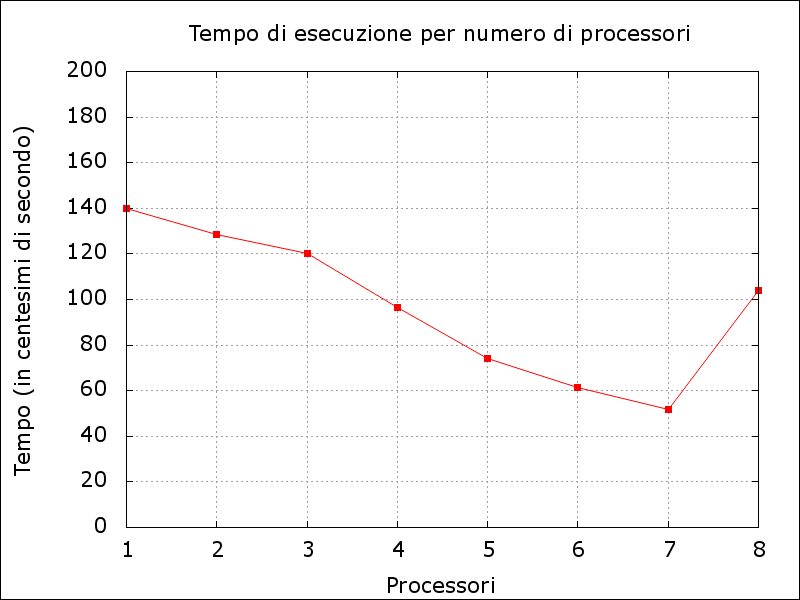
\includegraphics[width=0.8\textwidth]{grafico-tempi.png}
\end{center}
\caption{Grafico dei tempi di esecuzione al variare del numero di processori.}
\end{figure}

\begin{figure}[ht]
\begin{center}
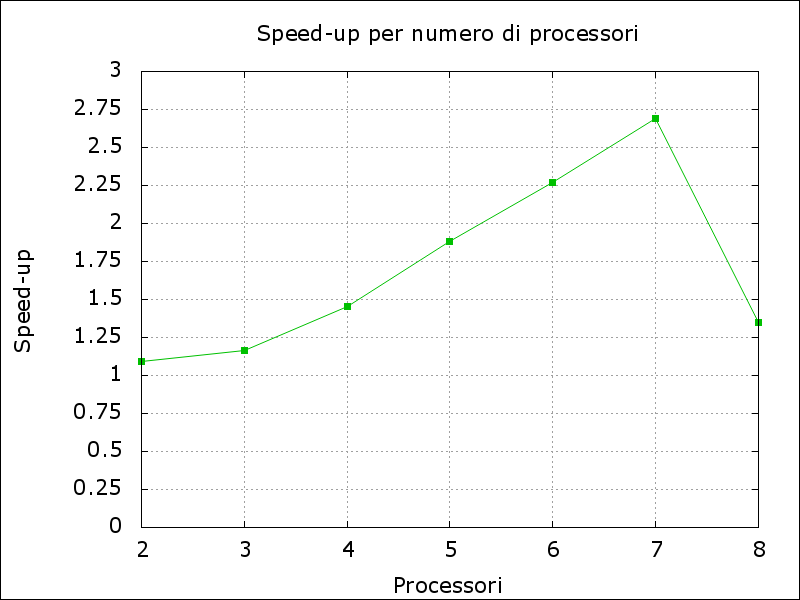
\includegraphics[width=0.8\textwidth]{grafico-speed-up.png}
\end{center}
\caption{Grafico dello speed-up al variare del numero di processori.}
\end{figure}

\begin{figure}[ht]
\begin{center}
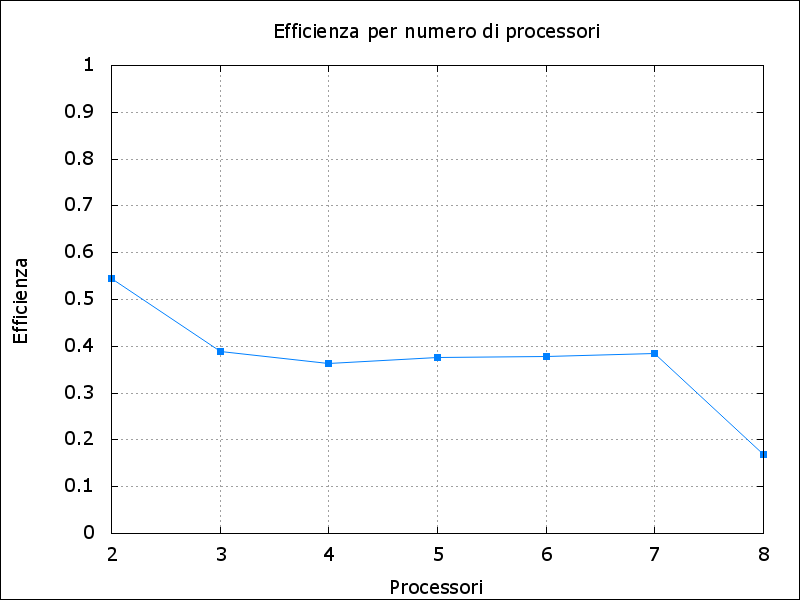
\includegraphics[width=0.8\textwidth]{grafico-efficienza.png}
\end{center}
\caption{Grafico dell'efficienza al variare del numero di processori.}
\end{figure}

Purtroppo la procedura DPLL \textit{dipende in maniera critica dai dati in ingresso}; qualora la formula favorisca l'applicazione delle regole che evitano lo sdoppiamento si hanno dei tempi di esecuzione molto rapidi, ma con l'aumentare degli sdoppiamenti si diverge rapidamente ed inesorabilmente\footnote{Salvo il caso in cui non venga scoperto un algoritmo che dimostri che $P=NP$.} verso l'esponenzialità dei tempi d'esecuzione rispetto al numero di variabili; ciò avviene perché il numero di processori a disposizione \textit{diventa rapidamente} insufficiente per esplorare in parallelo tutti i rami dell'albero degli assegnamenti.

L'istanza del problema SAT utilizzata per questa misura delle prestazioni, oltre al prevedibile basso incremento dei tempi d'esecuzione , ha causato un crollo degli stessi con un numero di processori superiore a 7; questo accade perché con la presenza dell'ottavo processore l'albero degli assegnamenti viene ripartito in maniera sfavorevole\footnote{Sfavorevole per quanto riguarda l'applicazione delle regole di semplificazione della procedura DPLL, ovviamente.} tra i vari worker ed il tempo per speso per le comunicazioni non è bilanciato da un calcolo del risultato particolarmente rapido.





\chapter{Conclusioni}

Per questo progetto sono previsti sviluppi futuri nell'ambito dell'insegnamento di Fondamenti di Intelligenza Artificiale.

Per quanto riguarda la parallelizzazione, il suo futuro è la \textit{modularità}: dovrà essere possibile aggiungere algoritmi diversi dalla DPLL che lavorino contemporaneamente ad essa ed abbiano un \textit{comportamento diverso}, possibilmente speculare rispetto agli stessi dati in ingresso. Proprio per favorire questa espandibilità, il progetto è stato scritto in C++ e strutturato con una minima architettura orientata agli oggetti.

Riguardo l'implementazione della procedura DPLL, particolare cura verrà posta nella creazione di \textit{euristiche} che permettano di scegliere la variabile su cui verrà effettuato lo sdoppiamento al fine di minimizzare la divergenza esponenziale dei tempi di esecuzione, poiché questa dipende in maniera critica proprio da tale operazione. Purtroppo però ad oggi non esistono euristiche totalmente affidabili.

Per quanto riguarda l'esperienza appena conclusa, questo progetto è stato particolarmente valido come esempio di \textit{portabilità}: grazie all'uso del linguaggio C++ e dello standard MPI 2 è stato possibile avere un programma funzionante allo stesso modo con compilatori ed implementazioni MPI differenti senza particolari problemi.






\end{document}

% That's all, folks!

